\chapter{Platforma od strony technicznej}
\label{chapter:platform-technical}
Ogólny schemat platformy wraz z użytymi technologiami został przedstawiony na rysunku \ref{fig:platform-schema}.

\begin{figure}[h]
    \centering
    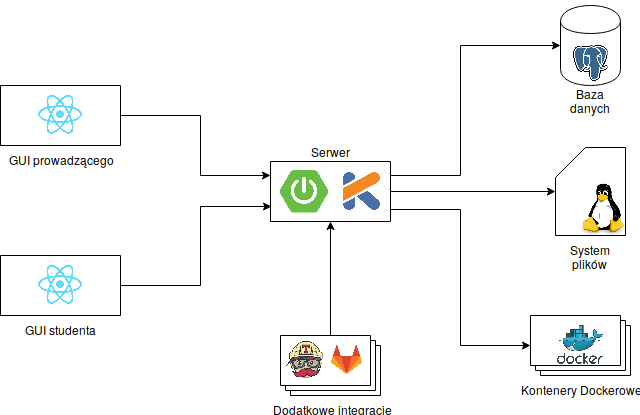
\includegraphics[width = 13cm]{chapter02/platform_schema.png}
    \caption{Schemat platformy i użytych technologii (źródło własne).}
    \label{fig:platform-schema}
\end{figure}

Platforma składa się z dwóch webowych interfejsów graficznych: interfejsu prowadzącego oraz studenta.
Oba interfejsy zostały napisane w technologii ReactJS z użyciem MaterialUI.

Moduł serwera został napisany w języku Kotlin z użyciem SpringBoot’a w wersji 2.0.

Serwer przechowuje dane w formie rekordów w bazie danych oraz plików.
Metadane, takie jak termin realizacji wskazanego etapu lub grupy, do których są przypisani studenci, są zapisywane w bazie PostgreSQL.
Schematy tabel i ich relacji zostały omówione w podrozdziale \ref{database}.
Dane w postaci plików są przechowywane na dysku serwera w systemie plików Linux.
W podrozdziale \ref{directories} opisano użyte struktury katalogów.

Programy studentów są uruchamiane w kontenerach Dockerowych.
Proces testowania aplikacji studentów został opisany w podrodziale \ref{run-and-test}.
Kolejna sekcja przedstawia utworzenie nowego środowiska uruchomieniowego w postaci Dockerfile.

Opis zastosowanej autoryzacji i autentykacji użytkowników można znaleźć w podrozdziale \ref{authorization}.

Przykład konfiguracji i uruchomienia platformy na dowolnym serwerze został omówiony w ramach sekcji \ref{run-platform}.

Platformę można zintegrować z zewnętrznymi narzędziami.
Przykładem takiej integracji może być repozytorium kodu oraz system CI (ang. Continious Integration).
System CI (Travis) można skonfigurować w taki sposób, aby bezpośrednio po zaakceptowaniu PR (ang. Pull Request) do repozytorium kodu (GitLab) uruchamiany był job, który po poprawnym zbudowaniu programu automatycznie przesyłał go do platformy i uruchamiał.
Przykład takiej integracji platformy z zewnętrznymi narzędziami został opisany w podrozdziale \ref{ci-integration}.

\section{Schemat bazy}
\label{database}

\begin{figure}[h]
    \centering
    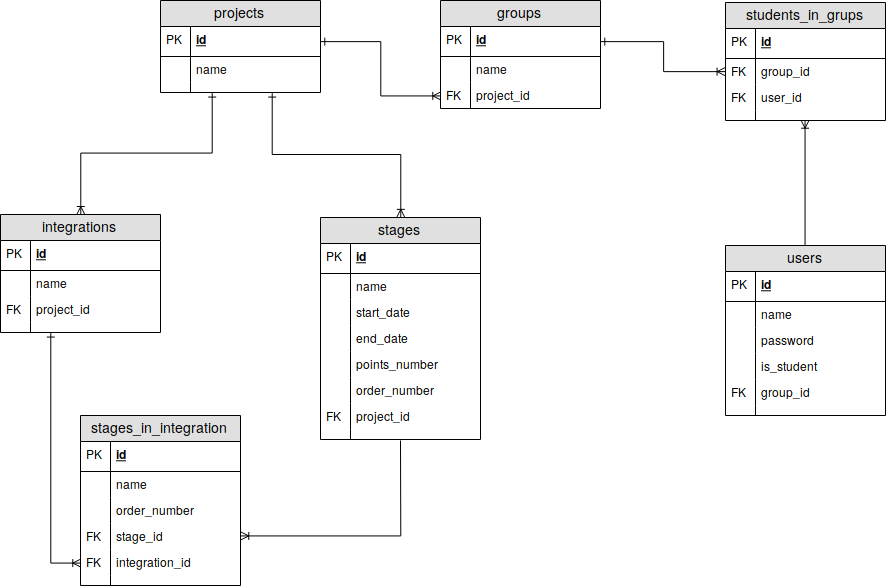
\includegraphics[width = 13cm]{chapter02/db_schema.png}
    \caption{Schemat bazy danych (źródło własne).}
    \label{fig:platform-db-schema}
\end{figure}

Schemat table i relacji bazodanowych, utworzony w ramach pracy, znajduje się na rysunku \ref{fig:platform-db-schema}.
Do przechowywania metadanych wykorzystano siedem tabel.
W przedstawionych strukturach przechowywane są informacje o:
\begin{itemize}
    \item istniejących projektach,
    \item grupach w ramach projektów,
    \item studentach w ramach grup,
    \item etapach w ramach projektów,
    \item integracjach w ramach projektów wraz z wykorzystywanymi do przeprowadzenia integracji etapami.
\end{itemize}

Do przechowywania danych użyto relacyjnej bazy PostgreSQL.
Pełne definicje tabel wraz z użytymi typami danych i więzami znajdują się w załączniku \ref{file:database-schema}.


\section{Schemat katalogów plików}
\label{directories}

Pełny schemat katalogów plików znajduje się na rysunku \ref{fig:platform-directories}.
Można wyróżnić na nim dwa podstawowe foldery: students oraz projects.
Wewnątrz pierwszego z nich zapisywane są wszystkie dane i pliki związane z aktywnością studentów zarejestrowaną na platformie.
Do zapamiętywanych informacji należą: raporty, linki do kodu, programy, logi z przebiegu aplikacji oraz wyniki przeprowadzonych testów akceptacyjnych.
Drugi folder zawiera definicje projektów wraz z etapami i integracjami oraz utworzone przez prowadzących przypadki testowe.

\begin{figure}[h]
    \centering
    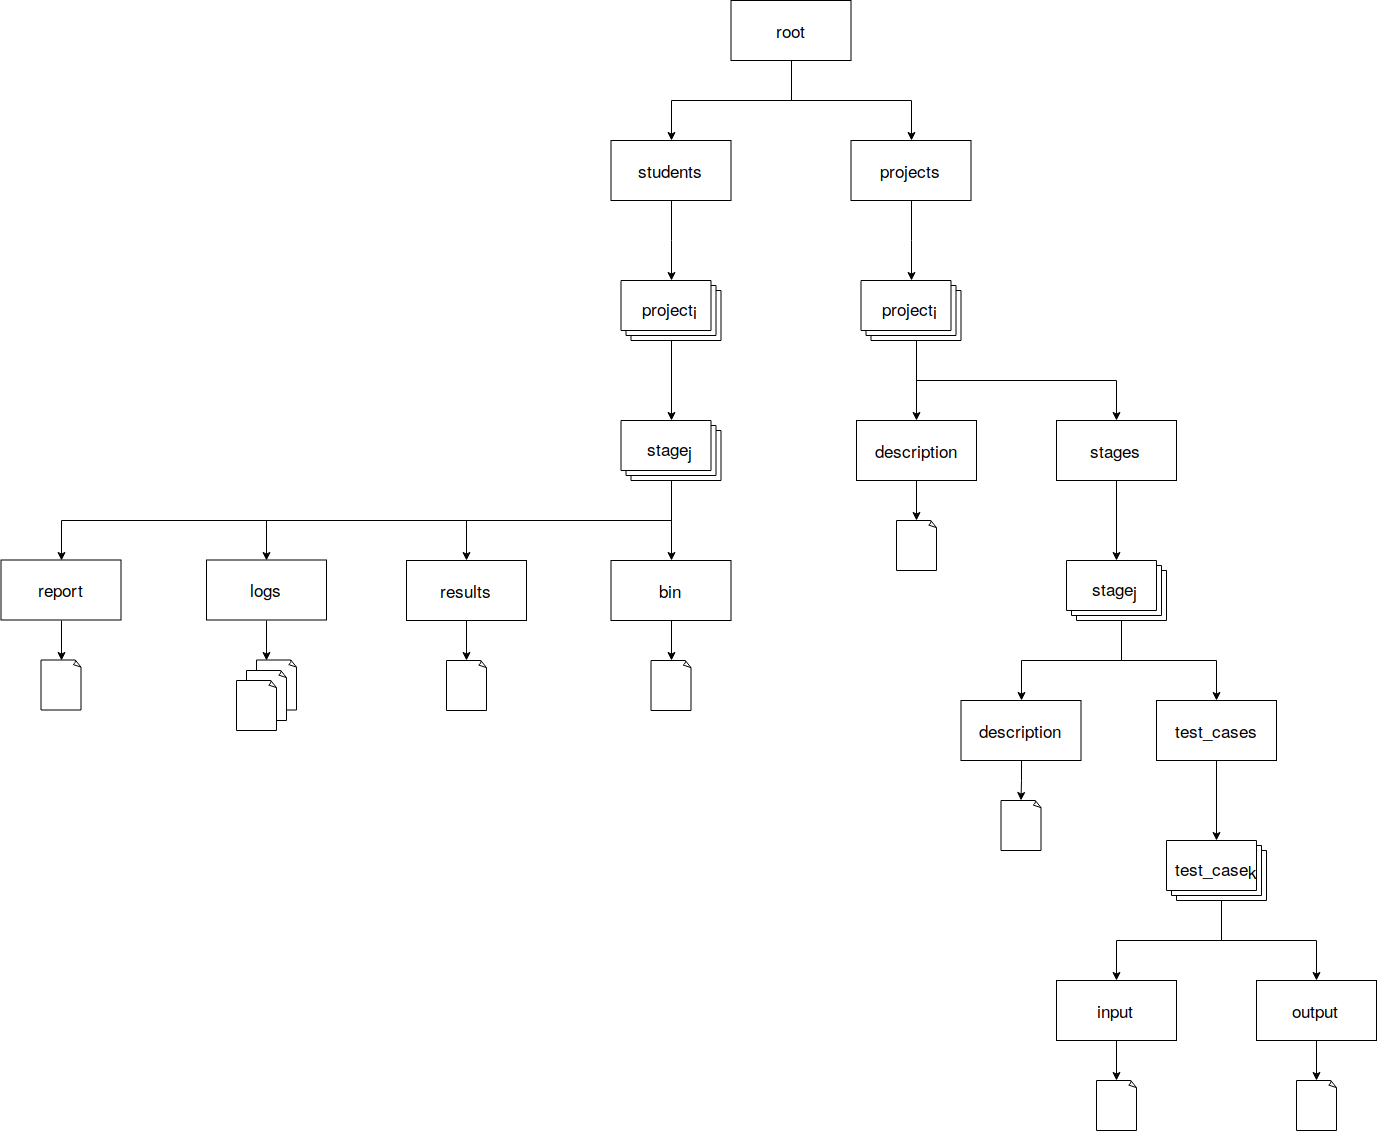
\includegraphics[width = 13cm]{chapter02/directories.png}
    \caption{Schemat katalogów plików (źródło własne).}
    \label{fig:platform-directories}
\end{figure}

\vfill

\section{Uruchomianie i testowanie programów studentów}
\label{run-and-test}

Programy studentów są uruchamiane w kontenerach Dockerowych.
Obraz środowiska jest ustalany dla zadanego projektu.
Technologia Docker jest szeroko używana komercyjnie.
Dzięki temu charakteryzuje się ona wysoką niezawodnością i stabilnością.
Również biblioteki OpenSource ułatwiające uruchamianie kontenerów Dockerowych bezpośrednio z kodu Javowego są szeroko stosowana i dobrze przetestowane.
Samo uruchamianie kontenerów, ich integracja oraz konfiguracja nowych środowiska, jest szybka i stosunkowo prosta.

\begin{figure}[h]
    \centering
    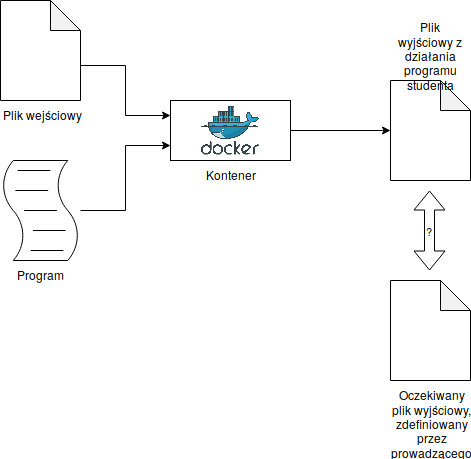
\includegraphics[width = 13cm]{chapter02/single_test_case.png}
    \caption{Schemat sprawdzenia poprawności działania programu studenta (źródło własne).}
    \label{fig:single-test-case}
\end{figure}

Schemat sprawdzenia poprawności działania programów studentów został przedstawiony na rysunku \ref{fig:single-test-case}.
Po uruchomieniu programu studenta na platformie, uruchamiane są wszystkie przypadki testowe dla zadanego etapu.
Uruchomienie pojedynczego przypadku testowego sprowadza się do utworzenia nowego kontenera Dockerowego i podania mu jako volumenu ścieżki do programu studenta oraz ścieżki do pliku wejściowego.
Program studenta jest uruchamiany dla zadanych danych wejściowych w kontenerze.
Oczekuje się, że program studenta w wyniku swojego działania utworzy plik wyjściowy.
Zawartość tego pliku zostanie porównana z zawartością oczekiwanego pliku wejściowego dla danego przypadku testowego. Jeśli dane są zgodne, przypadek testowy uważa się za spełniony.

\begin{figure}[h]
    \centering
    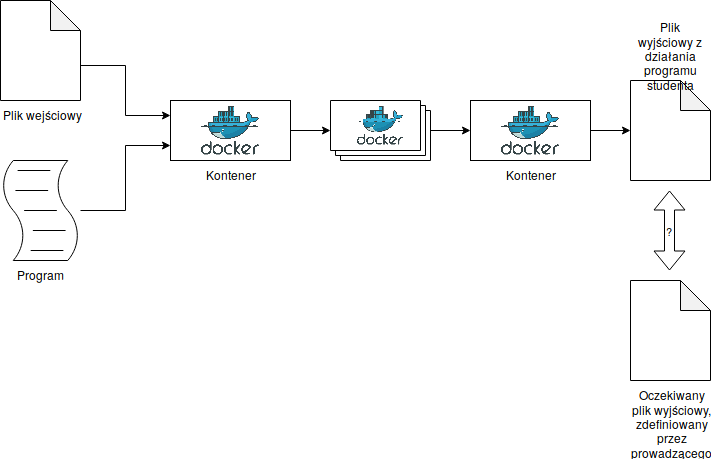
\includegraphics[width = 13cm]{chapter02/integration.png}
    \caption{Schemat sprawdzenia poprawności procesu integracji programów studentów (źródło własne).}
    \label{fig:integration}
\end{figure}

Schemat przebiegu procesu integracji został przedstawiony na rysunku \ref{fig:integration}.
Prowadzący definiuje kolejne etapy wykonywane w ramach procesu integracji.
Przebieg procesu integracji jest bardzo podobny do wykonania pojedynczego przypadku testowego.
Różnica polega na tym, że plik wyjściowy utworzony w wyniku uruchomienia poprzedniego etapu jest plikiem wejściowym dla kolejnego, następującego po nim.
Plik wyjściowy dla ostatniego etapu jest porównywany ze zdefiniowanym oczekiwanym plikiem wyjściowym.

\section {Konfiguracja uruchomieniowego środowiska Dockerowego}

TODO: Opis i przykład

\section {Uwierzytelnienie użytkowników}
\label{authorization}

TODO: opis:
1) proste uwierzytelnienie oparte o login i hasło
2)prosta autoryzacja oparta o nadanie praw administratora prowadzącym
oraz ograniczenie praw wykonania studentom,

\section {Zestawienie platformy na serwerze}
\label{run-platform}

TODO: Opis i przykład

\section {Przykład integracji platformy z narzędziem CI oraz repozytorium kodu}
\label{ci-integration}

TODO: opis i przykład integracji platformy z narzędziem CI oraz repozytorium
kodu.